\section{Experimentos}

\begin{frame}{Ambiente de Teste}
	\begin{itemize}
		\item https://www.emulab.net/
		\item Oito máquinas
		\begin{itemize}
			\item Três para o serviço de metadados
			\item Quatro para o serviço de armazenamento
			\item Uma para o cliente.
		\end{itemize}
	\end{itemize}
\end{frame}

\begin{frame}{Ambiente de Teste}
		\begin{table} [htb]
			\caption{Especificações Técnicas das Máquinas}
			\centering
			\begin{tabular}{|l|l|} \hline
				\textbf{Descrição} 	& \textbf{Valor} \\ \hline
				
				Tipo				& d430\\ \hline
				Classe				& PC\\ \hline
				Sistema Operacional & Ubuntu (64bits)\\ \hline
				Disco Rígido		& 200GB \\ \hline
				Memória RAM			& 4GB \\ \hline
				Nº de \textit{Cores}& 8 \\ \hline
				Velocidade do CPU	& 2.4GHz  \\ \hline
				
			\end{tabular}
			\label{tab:exp_vm}
		\end{table}
\end{frame}

\begin{frame}{Ambiente de Teste}
		\begin{figure}
			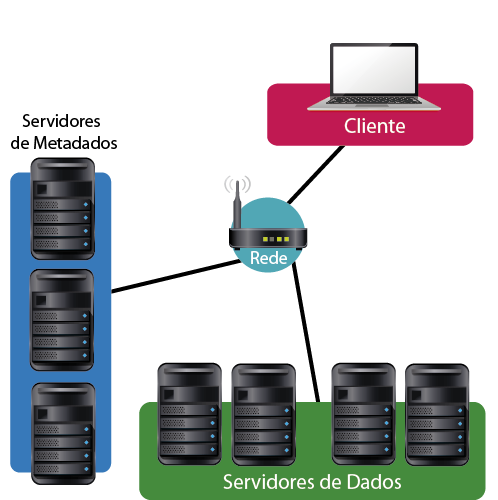
\includegraphics[width=5.5cm]{imagens/emulab}
			%\caption{Topologia da Rede}
			\label{fig:emulab}
		\end{figure}
	
\end{frame}

\begin{frame}{Teste de Latência}
	\begin{itemize}
		\item O objetivo do teste de latência é mensurar o tempo total que o sistema leva para executar uma operação.
		\item Operações
		\begin{itemize}
			\item Leitura
			\item Escrita
		\end{itemize}
		\item 1000 vezes consecutivas
		\item Tamanho dos Arquivos
		\begin{itemize}
			\item 1KB
			\item 100KB
			\item 1MB
			\item 10MB
		\end{itemize}
		\item Repetido para os três tipos de RAID.
	\end{itemize}
\end{frame}

\begin{frame}{Teste de Vazão}
	\begin{itemize}
		\item O objetivo do teste de vazão (ou \textit{throughput}) é mensurar quantas operações concorrentes o sistema consegue executar por segundo.
		\item Similar ao teste de latência, porém com a adição de clientes enviando solicitações em paralelo.
		\item Uma máquina cliente utilizando múltiplas \textit{threads}.
		\begin{itemize}
			\item 10 \textit{threads}
			\item 20 \textit{threads}
			\item ...
			\item 50 \textit{threads}
		\end{itemize}
	\end{itemize}
\end{frame}